\documentclass[
	a4paper, % Paper size, use either a4paper or letterpaper
	10pt, % Default font size, can also use 11pt or 12pt, although this is not recommended
	unnumberedsections, % Comment to enable section numbering
	twoside, % Two side traditional mode where headers and footers change between odd and even pages, comment this option to make them fixed
]{LTJournalArticle}

\addbibresource{sample.bib} % BibLaTeX bibliography file

% A shortened article title to appear in the running head, leave this command empty for no running head

% \footertext{\textit{Journal of Biological Sampling} (2024) 12:533-684} % Text to appear in the footer, leave this command empty for no footer text

\setcounter{page}{1} % The page number of the first page, set this to a higher number if the article is to be part of an issue or larger work

%----------------------------------------------------------------------------------------
%	TITLE SECTION
%----------------------------------------------------------------------------------------

\title{Enhancing Search Precision With Embeddings-Based Semantics} % Article title, use manual lines breaks (\\) to beautify the layout

% Authors are listed in a comma-separated list with superscript numbers indicating affiliations
% \thanks{} is used for any text that should be placed in a footnote on the first page, such as the corresponding author's email, journal acceptance dates, a copyright/license notice, keywords, etc
\author{%
	Adarsh Hiremath \\
	NEUROBIO 240: Biological and Artificial Intelligence \\
	ahiremath@college.harvard.edu
}


%----------------------------------------------------------------------------------------

\begin{document}

\maketitle % Output the title section

%----------------------------------------------------------------------------------------
%	ARTICLE CONTENTS
%----------------------------------------------------------------------------------------

\section{1. Introduction}

Embeddings are numerical representations of words, phrases, or documents that capture their semantic meaning in a vector space. They are commonly used in natural language processing applications, including search, recommendation systems, and sentiment analysis. In search, embeddings can efficiently and accurately retrieve relevant documents or web pages based on the similarity of their semantic content to the user's query.

In December 2022, OpenAI released its newest embedding model, \texttt{text-embedding-ada-002}. Open AI claims that \texttt{text-embedding-ada-002} is far more powerful similar models like BERT. However, little work has been done to quantify the differences between \texttt{text-embedding-ada-002} and more traditional approaches to search. In this paper, I intend to better quantify these differences by doing the following: 
\begin{itemize}
	\item Implementing search with \texttt{text-embedding-ad}
	\texttt{a-002}, BERT, and fuzzy matching. 
	\item Creating a custom dataset of my.Harvard classes and their corresponding data.
	\item Applying those searches to the my.Harvard dataset.
	\item Quantifying the differences between each search method. 
	\item Building a web application to search Harvard classes and releasing it to the Harvard community. 
\end{itemize}

\section{2. Literature Review}

Literature in the field of text embeddings for information retrieval is largely isolated to individual methods, with little work done to compare the effectiveness of different approaches. My paper aims to address this gap by evaluating the performance of three different search methods: \texttt{text-embedding-ada-002}, BERT, and fuzzy matching. From my literature review, I drew on the following papers the most: 


\begin{itemize}
	\item \textit{Text and Code Embeddings by Contrastive Pre-Training} (Neelakantan et al. 2022): an evaluation of unsupervised text embedding models on large-scale semantic search. These researchers measured an improvement of 23.4, 14.7, and and 10.6 percent over MSMARCO, Natural Questions and TriviaQA benchmarks. 
	\item \textit{Neural Text Embeddings for Information Retrieval} (Mitra and Craswell 2017): an overview of text embeddings pre-\texttt{davinci} for natural language tasks and information retrieval. 
	\item \textit{Semantic Search With Sentence-BERT for Design Information Retrieval} (Walsh and Andrade 2022): an overview of sentence-BERT, a modification to BERT that uses siamese networks for sentence embeddings. 
\end{itemize}

The Neelakantan paper forms the basis for my \texttt{text-embedding-ada002} implementation of semantic search. This paper asserts that it is possible to use a single embedding model to do large-scale semantic search. In my experiments, I use \texttt{text-embedding-ada002}  as the single embedding model for semantic search and evaluate it on the my.Harvard classes dataset. 

The Mitra and Craswell paper provided important context about embeddings in general and was helpful for my general understanding of embeddings.

Finally, the Walsh and Andrade paper was greatly helpful for my initial work on the implementation of the BERT-based search. The insighit of passing in the text through a siamese network to determine similarity was particularly helpful. 

\section{3. Dataset}

Several datasets exist for text classification and  aggregation. Initially, I considered testing my semantic search functionality on the following: 
\begin{itemize}
	\item \textit{MS MARCO}: a text dataset with over $1,000,000$ queries and their corresponding saerch results from the Bing search engine. It is commonly used for passage retrieval. 
	\item \textit{The Reuters Corpus}: a text dataset with over $10,000$ articles from Reuters, labeled with categoreis such as "earnings" and "acquisitions."
	\item \textit{CORD-19}: a dataset with over $200,000$ scholarly articles related to COVID-$19$ and other coronaviruses. It is commonly used for information retrieval.
\end{itemize}

However, none of these datasets had queries pre-labeled with "ground truth" about how relevant search responses were. Instead of manually labeling the relevance of search queries for datasets I was unfamiliar with, I opted to use a custom dataset of my.Harvard classes. This dataset contains over $8000$ my.Harvard classes organized in the following JSON format: 

\begin{python}
	{
		"Id": "G0EnBh8",
		"Subject": "AFRAMER",
		"Number": "11",
		"ClassNumber": "13878",
		"CourseId": "123591",
		"Name": "Introduction to African 
		Studies",
		"Desc": "<p>This course introduces 
		students to the rich diversity and 
		complexity of Africa, including 
		its historical dynamics, 
		economic developments, ...",
		"Profs": "Daniel Agbiboa",
		"F22": true,
		"Days": [
		"Th"
		],
		"M": "N",
		"T": "N",
		"W": "N",
		"R": "Y",
		"F": "N",
		"StartTime": "9:45am",
		"EndTime": "11:45am",
		"HasSection": true,
		"Prereq": "Required of 
		concentrators in African 
		Studies track.",
		"SOC": true,
		"Exam": "12/09/2022 2:00 PM",
		"Location": "Cambridge",
		"URL": "https://locator.
		tlt.harvard.edu/course/
		colgsas-123591/2022/fall/13878",
		"AcadOrg": [
		"AAAS",
		"HIST",
		"EMR"
		]
	}
\end{python}

Given that my.Harvard's native search only works with ultra-precise search queries for course titles and course names, applying semantic search to my.Harvard classes appeared to be a far more useful and relevant use case for the Harvard community.

my.Harvard has no consistency for the JSON representing each class, making the scraping operation extremely difficult. For help with generating the dataset, I reached out to the creator of Deez Classes. 

\section{4. Search Implementations}

Each search technique varies in implementation. \texttt{text-embedding-ada-002}, a transformer-based deep learning architecture is utilized along with cosine similarity to measure query and text similarity. The BERT search is implemented using a custom tokenizer, while fuzzy matching uses string-matching algorithms to return results according to a given threshold.

\subsection{4.1 text-embedding-ada-002}

OpenAI's embedding model, \texttt{text-embedding-ad} 
\texttt{a-002}, utilizes a transformer-based deep learning architecture to learn  embeddings. \texttt{text-embedding-ada-002} outperforms the other top models in three standard benchmarks and is useful for working with natural language and code. Semantically similar text is also numerically similar, and the new embeddings endpoint in the OpenAI API provides easy access to the model used to generate embeddings. Although OpenAI offers three families of embedding models - text embeddings text search / similarity, and code search - I only used the base text embedding model for my project.


\begin{figure}[h]
    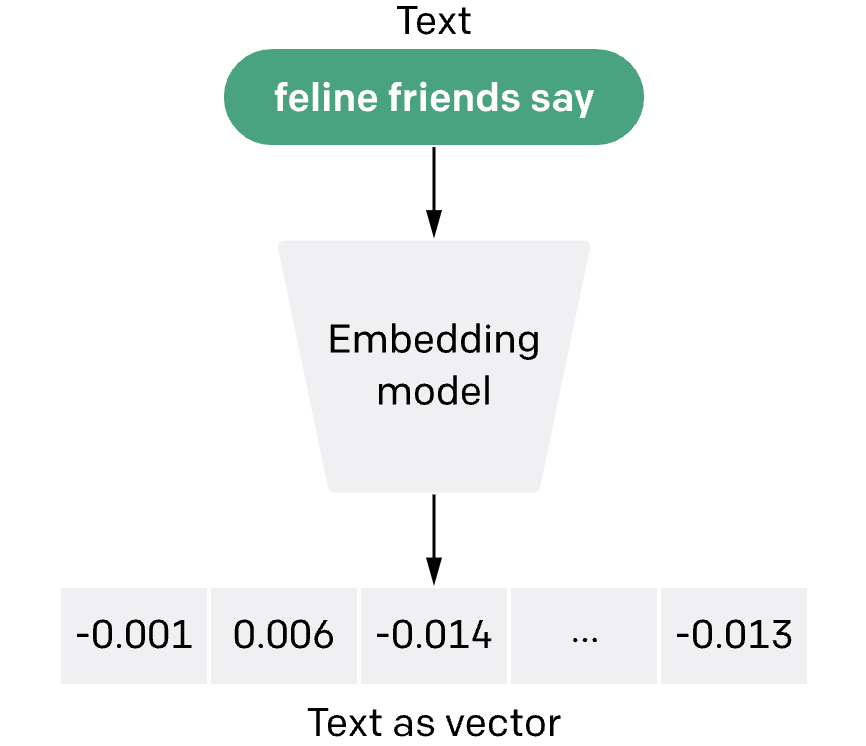
\includegraphics[width=8.1cm]{embedding.png}
    \caption{An example of text embeddings in a vector space.}
    \label{fig:embedding}
\end{figure}


I wanted my search to correctly identify classes based on their name, description, professors, start time, and end time. So, in a Pandas dataframe, I combined all of this information into a column called "combined." From there, generating the embedding was straightforward and required making a call to OpenAI's \texttt{text-embedding-ada-002} endpoint as follows: 

\begin{python}
	course["combined"] = "Title: " + 
	course["Name"] + "; Description: " + 
	course["Desc"] + "; Professors: " + \
	course["Profs"] + "; StartTime: " + \
	course["StartTime"] + "; EndTime: " + 
	course["EndTime"]

	course["embedding"] = 
	openai.Embedding.create(
	input=course["combined"], 
	engine="text-embedding-ada-002")
	["data"][0]["embedding"]
\end{python}

Initially, I considered combining the individual embeddings for the course name, description, professors, start time, and end time to increase the accuracy of my search with a custom formula. However, I decided against this for a couple reasons: 
\begin{itemize}
	\item Dimensionality: it was challenging to combine embeddings because their high dimensionality added an additional alignment step before making meaningful comparisons.
	\item Computational expenses: combining embeddings required calling the Open AI API and doing cosine similarity more times, increasing the cost and time of the algorithm. 
	\item Context: several papers indicated that embeddings can be sensitive to context, leading to variability in their quality and usefulness for different search tasks. Thus, combining embeddings from different sources or models can result in inconsistent or noisy results.
\end{itemize}


\subsection{4.2 BERT}

Just like for the \texttt{text-embedding-ada-002} approach, implementing the BERT search required a similar set of steps: make a combined column, encode the text, and return results by cosine similarity. However, unlike  \texttt{text-embedding-ada-002}, BERT required some additional modifications to work properly. 

BERT expects input in a specific format, where each token is mapped to a unique integer ID, and special tokens are added to denote the start and end of the input sequence. Therefore, before encoding the text using BERT, I need to tokenize the text and convert the tokens to their corresponding integer IDs.

My bert\_encode function uses a custom tokenizer that is specifically designed for the course description data used in this project. The tokenizer is created by combining several standard tokenization techniques, such as lowercasing, removing stop words, and splitting on punctuation marks. Additionally, I include some domain-specific tokenization techniques to handle course codes and titles, such as splitting on parentheses, forward slashes, and colons. This helped to improve the accuracy of the BERT embeddings and, therefore, the quality of the search results.


\subsection{4.3 Fuzzy Matching}

To compare my transformer-based search approaches to a more traditional search algorithm, I also implemented a fuzzy matching search algorithm using Levenshtein distance. Levenshtein distance is a string metric used to measure the difference between two sequences and is calculated as the minimum number of single-character edits (insertions, deletions, or substitutions) required to transform one string into the other. 

\begin{figure}[h]
    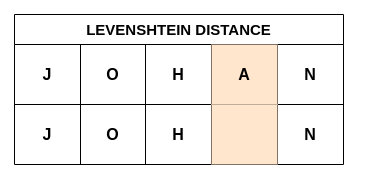
\includegraphics[width=8.1cm]{fuzzy.png}
    \caption{Fuzzy matching with Levenshtein Distance.}
    \label{fig:fuzzy}
\end{figure}

Fuzzy matching with Levenshtein distance involves comparing a search query to a set of strings and returning the closest matches based on their Levenshtein distance. The algorithm works by calculating the Levenshtein distance between the search query and each string in the set. The strings with the smallest Levenshtein distance are considered the closest matches and are returned as search results.

In my search algorithm, I used the following Python implementation of fuzzy matching with structural modifications to calculate the Levenshtein distances between the search query and the class data:

\begin{python}
	import numpy as np
	from Levenshtein import distance

	def fuzzy_match(query, strings, threshold):
		distances = np.array([distance(query, s)
		 for s in strings])
		matches = [s for i, s in 
		enumerate(strings) if 
		distances[i] <= threshold]
		return matches
\end{python}

In the following example, the fuzzy\_match function returns a list of strings from \texttt{strings} that are closest to \texttt{query} based on their Levenshtein distance:

\begin{python}
	query = "Harvard"
	strings = ["Harvrd", "Havard", 
	"Harvad", "Havrd", "Harvardd", "Hrvard"]
	threshold = 2

	matches = [s for s in strings 
	if distance(query, s) < threshold]
	print(matches)
\end{python}

The algorithm will only return "Harvrd," "Havard," and "Harvad" because they are all distance $1$ away from the original query. Conversely, "Havrd" and "Hrvard" will not be returned because they are distance $2$ away from the original query.

While Levenshtein distance is a great matching technique for smaller queries and search text, the distance metric fails for larger search text (like Harvard class data), which will be shown later on in this paper. 

\section{5. Result Sampling}

Before quantifying the differences in search techniques numerically, I wanted to document notable search-response results for each search technique to confirm the notion that an embeddings-based search would be better than naive approaches.

\subsection{5.1 text-embedding-ada-002}

Unlike my.Harvard's native search, \texttt{text-embeddi}
\texttt{ng-ada-002} is exceptional at dealing with search queries that don't directly correspond with course names or contain spelling errors. To illustrate the power of embeddings-based semantics, we examine a couple examples:



\begin{figure}[h]
	\begin{center}
		\texttt{Query:} \\
		\texttt{I want to take classes about African Studies with an emphasis on Christianity or culture.} \\
		\texttt{}\\
		\texttt{Output:} 
		\begin{itemize}
			\item \texttt{Christianity, Identity and Civil Society in African}
			\item \texttt{Introduction to African Studies}
			\item \texttt{Introduction to African American Studies}
		\end{itemize}		
	\end{center}

	\caption{An example query to the \texttt{text-embedding} \texttt{-ada-002} search engine. Although class descriptions are used for the search responses, they are omitted for length. Additionally, the results are ranked in descending order based on relevance. Only 3 responses are returned per query.}
	\label{fig:ex1}
\end{figure}


The OpenAI-enabled search engine returned three relevant search results, sorted from most to least relevant. The class descriptions for Christianity, Identity and Civil Society in African matched the search query most heavily, while Introduction to African Studies had a class description that aligned more similarly with the search query than Introduction to African American Studies.  

To verify whether the OpenAI-enabled approach truly has semantic understandings of search queries, we can even replace most words in the search query with a synonym and obtain similar performance: 

\begin{figure}[h]
	\begin{center}
		\texttt{Query:} \\
		\texttt{I would be interested in taking courses about African Learnings with an priority on Catholicism or culture.} \\
		\texttt{}\\
		\texttt{Output:} 
		\begin{itemize}
			\item \texttt{Introduction to African Languages and Cultures}
			\item \texttt{Christianity, Identity and Civil Society in African}
			\item \texttt{African Literature and Culture Since 1800}
		\end{itemize}		
	\end{center}

	\caption{An example query to the \texttt{text-embedding} \texttt{-ada-002} search engine. Although class descriptions are used for the search responses, they are omitted for length. Additionally, the results are ranked in descending order based on relevance. Only 3 responses are returned per query.}
\end{figure}

While slightly different, the search engine returns highly relevant results when given a search query modified with synonyms. However, unlike the embeddings-based approach, my.Harvard's native functionality fails with similar queries. This is easily verifiable by inputting the same search query into my.Harvard: 


\begin{figure}[h]
	\begin{center}
		\texttt{Query:} \\
		\texttt{I want to take classes about African Studies with an emphasis on Christianity or culture.} \\
		\texttt{}\\
		\texttt{Output: }\\
		\texttt{No results found. Please refine your search and try again.}		 
	\end{center}
	\caption{An example query to my.Harvard's native search engine.}
	\label{fig:ex2}
\end{figure}


The \texttt{text-embedding-ada-002} approach is highly effective in understanding search semantics, even when there are spelling errors in the search query. In fact, modifying the previous search query with spelling errors results in a response that is nearly identical.

\begin{figure}[h]
	\begin{center}
		\texttt{Query:} \\
		\texttt{I wnt take clss abt African Stds with emphs on Christianity or culture.} \\
		\texttt{}\\
		\texttt{Output:} 
	\end{center}
\end{figure}

\begin{figure}
	\begin{center}
		\begin{itemize}
			\item \texttt{Christianity, Identity and Civil Society in African}
			\item \texttt{Introduction to African Popular Culture}
			\item \texttt{Introduction to African American Studies}
		\end{itemize}		
	\end{center}

	\caption{An example query to the \texttt{text-embedding} \texttt{-ada-002} search engine. Although class descriptions are used for the search responses, they are omitted for length. Additionally, the results are ranked in descending order based on relevance. Only 3 responses are returned per query.}
\end{figure}


The embeddings model overweights for words spelled correctly, which is why the previously second ranked response is removed in favor of "Introduction to African Popular Culture" when "culture" is one of the only words in the search query that is spelled correctly. 

For my.Harvard's search, replacing even one character from the course title results in an invalid search query. Here, we search directly for the class name with but spell "Christianity" as "Christinity": 


\begin{figure}[h]
	\begin{center}
		\texttt{Query:} \\
		\texttt{Christinity, Identity and Civil Society in African.} \\
		\texttt{}\\
		\texttt{Output: } \\
		\texttt{No results found. Please refine your search and try again. }\\
	\end{center}
	\label{fig:ex4}
	\caption{An example query to my.Harvard's native search engine.}
\end{figure}


Ultimately, without even conducting any numerical tests, it is already clear that an embeddings-based approach is far more powerful than search protocols implemented in many contexts, including my.Harvard. 

\subsection{5.2 BERT}

Like the \texttt{text-embedding-ada-002} 
approach, we also expect BERT to perform far better than my.Harvard's native search. However, qualitative results indicate that there is a marked difference between BERT and \texttt{text-embedding-ada-002} in terms of performance. First, repeating the previous specific search query about classes about African studies shows noisier results for the top $3$ responses: 

\begin{figure}[h]
	\begin{center}
		\texttt{Query:} \\
		\texttt{I want to take classes about African Studies with an emphasis on Christianity or culture.}\\
		\texttt{}\\
		\texttt{Output:}
	\end{center}
\end{figure}

\begin{figure}
	\begin{center}
		\begin{itemize}
			\item \texttt{Methods of Behavioral Research}
			\item \texttt{Methods of Behavioral Research}
			\item \texttt{Ancient Greek Political Thought}
		\end{itemize}		
	\end{center}

	\caption{An example query to the BERT search engine. Although class descriptions are used for the search responses, they are omitted for length. Additionally, the results are ranked in descending order based on relevance. Only 3 responses are returned per query.}
	\label{fig:ex6}
\end{figure}


While the OpenAI-enabled search engine returned three relevant search results, sorted from most to least relevant, the BERT search approach did not return any relevant responses for the exact same search query about African Studies classes with an emphasis on Christianity or culture. This indicates that the BERT approach is less effective in understanding search semantics compared to the embeddings-based approach. 

While unreliable, BERT search does handle some search queries exceptionally well. For instance, take the following example for a query for discrete mathematics classes:

\begin{figure}[h]
	\begin{center}
		\texttt{Query:} \\
		\texttt{Discrete mathematics for computer science majors.} \\
		\texttt{}\\
		\texttt{Output:} 
		\begin{itemize}
			\item \texttt{Studies in Real and Complex analysis}
			\item \texttt{Discrete Mathematics for Computer Science}
			\item \texttt{Studies in Algebra and Group Theory}
		\end{itemize}		
	\end{center}
	\caption{An example query to the BERT search engine. Although class descriptions are used for the search responses, they are omitted for length. Additionally, the results are ranked in descending order based on relevance. Only 3 responses are returned per query.}
\end{figure}

This example clearly illustrates the power of semantics. Although "discrete mathematics" is nowhere to be found within the course titles or descriptions for two of the responses, the embeddings model is able to associate "discrete mathematics" with semantically similar topics such as "abstract algebra." 

Although BERT is a powerful model, it may not be the best choice for semantic search due to its inconsistency. OpenAI's embeddings approach achieves similar performance on the above search queries (including the discrete mathematics example) without the inconsistency of BERT. There could be several reasons why BERT may be less effective at semantic search than Open AI's embeddings model. 

\begin{itemize}
	\item  BERT is a far more contextual model that relies on the surrounding words to understand the meaning of a word, whereas \texttt{text-embedding-ada-002} does not require as much context to generate a fixed vector representation of words or phrases. 
	\item BERT is trained on less text than text-embedding-ada-002, which can lead to BERT being less effective at identifying the most relevant information for a given search query.
\end{itemize}

\subsection{5.3 Fuzzy Matching}


While the Levenshtein fuzzy matching approach performs well on small bodies of text such as just the course name, it fails to produce relevant results when searching through the entire body of text (course name, course description, and professor name) or when there are spelling errors. This is in contrast to the OpenAI embeddings-based approach and BERT, which are highly effective in understanding search semantics, even when there are spelling errors in the search query or the body of text to be searched is extremely large. 


\begin{figure}[h]
	\begin{center}
		\texttt{Query:} \\
		\texttt{I want to take classes about African Studies with an emphasis on Christianity or culture.} \\
		\texttt{}\\
		\texttt{Output:} 
		\begin{itemize}
			\item \texttt{Christianity, Identity and Civil Society in African}
			\item \texttt{Introduction to African Studies}
			\item \texttt{Introduction to African American Studies}
		\end{itemize}		
	\end{center}

	\caption{An example query to the \texttt{text-embedding} \texttt{-ada-002} search engine. Although class descriptions are used for the search responses, they are omitted for length. Additionally, the results are ranked in descending order based on relevance. Only 3 responses are returned per query.}
	\label{fig:ex1}
\end{figure}


% \section{6. Performance Metrics}

% \subsection{7.1 Speed}

% \subsection{7.2 Normalized Discounted Cumulative Gain (NDCG)}

% \subsection{7.3 Code Readability and Implementation}

% \section{8. Conclusions and Future Directions}

\end{document}
